\chapter{Résultats préliminaires dans un graphe circulaire à $n$ sommets}
\label{Résultats préliminaires}

\section{Inégalité ``triangulaire'' sur les coûts des arêtes}
\label{sec: Inégalité triangulaire}

On se donne un graphe $G=(V,E)$ circulaire à $n$ sommets et un coût $\bs{c} \in \RR^E_+$. On peut alors faire l'hypothèse suivante :
\begin{gather}\label{Inégalité Triangulaire}
  c_{e'}<\sum_{e \in E \backslash \{e'\}} c_e \quad \text{pour tout } e' \in E
\end{gather}

En effet, supposons qu'il existe $e' \in E$ tel que $c_{e'} \ge \sum_{e \in E \backslash \{e'\}} c_e$.

On se donne une solution optimale $(z_e)_{e \in E}$. Le coût d'une telle solution s'écrit $\Upsilon_{G}~=~\sum_{e \in E}~c_ez_e$. On construit alors la séquence de mouvement $(z'_e)_{e \in E}$ par le procédé suivant : chaque passage par l'arête $e'$ est remplacé par un passage sur les autres arêtes avec le même nombre de vélos. Autrement dit, ``on fait le tour dans l'autre sens''. On note $\Gamma'$ le coût d'une telle séquence. On a alors :
\begin{align*}
  \Gamma' &= \sum_{e \in E \backslash \{e'\}} c_e (z_e + z_{e'}) = \sum_{e \in E \backslash \{e'\}} c_ez_e + \left(\sum_{e \in E \backslash \{e'\}} c_{e}\right)z_{e'} \\
     &\le \sum_{e \in E \backslash \{e'\}} c_ez_e + c_{e'}z_{e'} = \Upsilon_{G}
\end{align*}

Par conséquent, il existe une solution au moins aussi bonne ne passant pas par $e'$. Pour obtenir la solution optimale, il suffit alors de résoudre le cas du graphe linéaire sur le graphe $G'$ obtenu en supprimant l'arête $e'$ du graphe $G$.

\section{Borne inférieure de la solution optimale (valable pour un graphe quelconque)}
\label{Borne inf générale}

Nous nous contentons ici de redonner la borne inférieure trouvée par les auteurs de l'article \cite{Benchimol2011}.
\\

Une borne inférieure du SSBP est la solution optimale du programme mathématique en nombres entiers dont les variables ``comptent'' le nombre de fois où le camion passe par chaque arête. Les contraintes sont les suivantes :
\begin{enumerate}[label=(\roman*)]
\item les variables sont des entiers naturels.
\item la condition d'Euler : sauf peut-être en $p$ et en $q$, le camion entre et sort de tout sommet un nombre paire de fois.
\item ``subtour elimination'' : si le camion est en $p \in U \subseteq V $ et qu'il existe des stations non-équilibrées dans $\overline{U}$, alors le camion doit nécessairement traverser $\delta(U)$ au moins une fois (voire plus, suivant la position de $q$). Nous utiliserons la notation suivante pour écrire cette contrainte :
\[
\mu(p,q,U,\bs{x},\bs{y}) = \left\{
\begin{array}{ll}
  0 &\mbox{ si } p,q \in U            \mbox{ et } \overline{U} \subseteq B(\bs{x},\bs{y})\\
  0 &\mbox{ si } p,q \in \overline{U} \mbox{ et } U \subseteq B(\bs{x},\bs{y})\\
  1 &\mbox{ si } p \in U              \mbox{ et } q \in \overline{U}\\
  1 &\mbox{ si } p \in \overline{U}   \mbox{ et } q \in U\\
  2 &\mbox{ si } p,q \in U            \mbox{ et } \overline{U} \backslash B(\bs{x},\bs{y}) \ne \emptyset\\
  2 &\mbox{ si } p,q \in \overline{U} \mbox{ et } U \backslash B(\bs{x},\bs{y}) \ne \emptyset
\end{array}
\right.
\]
\item Contrainte de capacité : si $U \subseteq V$ a trop de vélos, le camion doit quitter suffisament de fois $U$ afin de sortir tous ces vélo. Une notation utile est la suivante :
\[
\eta(p,q,U) = \left\{
\begin{array}{ll}
  -1 &\mbox{ si } p \in U            \mbox{ et } q \in \overline{U}\\
  0  &\mbox{ si } p \in U            \mbox{ et } q \in U\\
  0  &\mbox{ si } p \in \overline{U} \mbox{ et } q \in \overline{U}\\
  +1 &\mbox{ si } p \in \overline{U} \mbox{ et } q \in U\\
\end{array}
\right.
\]
\end{enumerate}

Cette borne inférieure est donc solution du programme mathématique en nombres entiers
\begin{gather}\label{PLNE borne inf}
\begin{array}{llll}
  \mbox{Min}_{\bs{z}} &\sum_{e \in E} c_ez_e & & \\
  \mbox{s.c.}       &z_e \in \ZZ_+ &\mbox{pour tout } e \in E &\mbox{(i)} \\
                    &z(\delta(v)) \mbox{ est paire} &\mbox{pour tout } v \in V \backslash \{p,q\}&\mbox{(ii)} \\
                    &z(\delta(U)) \ge \mu(p,q,U,\bs{x},\bs{y}) &\mbox{pour tout } U \subseteq V, U \ne \emptyset &\mbox{(iii)} \\
                    &z(\delta(U)) \ge 2 \left\lceil \frac{x(U)-y(U)}{C} \right\rceil\ + \eta(p,q,U) &\mbox{pour tout } U \subseteq V, U \ne \emptyset &\mbox{(iv)}
\end{array}
\end{gather}

\section{Un exemple où la borne inférieure n'est pas atteinte}

\begin{figure}[ht]
  \label{Exemple de borne inf non atteinte}
  \center 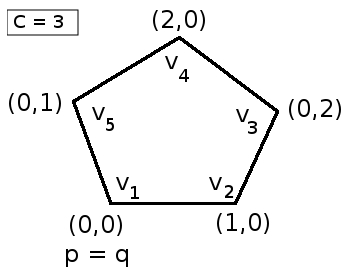
\includegraphics[scale=0.5]{BorneInfNonAtteinte-5sommets.jpg}
  \caption{Exemple de graphe circulaire à 5 sommets où la borne inférieure n'est pas atteinte}
\end{figure}

La solution du programme mathématique en nombre entier \eqref{PLNE borne inf} est $z_e = 1$, pour tout $e \in E$. C'est-à-dire qu'il suffirait de faire un tour complet du graphe sans revenir sur ses pas pour l'équilibrer. Or on constate qu'un tel parcours ne peut pas équilibrer le graphe.

Si dans certains cas particuliers du graphe circulaire, on peut utiliser l'égalité avec la borne inférieure solution du programme mathématique \eqref{PLNE borne inf}, on sait que dans le cas général cette méthode n'aboutira pas. En effet, on vient de montrer qu'il existe des cas où cette borne inférieure n'est pas atteinte.

\section{Changement de variables}
\label{Changement variables}

La description de la borne inférieure dans la section \ref{Borne inf générale} donne un minorant de $z(\delta(U))$ pour toute coupe $\delta(U)$ dans le graphe. Dans le cas de l'arbre décrit dans l'article \cite{Benchimol2011}, on avait donc un minorant de $z_e$ pour tout $e \in E$. Comme $c_e$ est positif pour tout $e\in E$, il suffisait de montrer que le minimum de $z_e$ était atteint pour tout $e \in E$ pour montrer que le coût $\sum_{e \in E}c_ez_e$ était minimal.

\begin{prop}\label{Parité coupe}
Soit $G=(V,E)$ un graphe dont tous les sommets sont de degrès paire. Alors toute coupe de G est de cardinal paire.
\end{prop}

\begin{proof}
Soit $U \subseteq V$. On note $E[U]$ l'ensemble des arêtes de $E$ ayant leur deux sommets dans $U$.
$$
\sum_{v \in U} deg(v) = \sum_{e \in E}\Indic_{\delta(U)}(e)  + 2 \sum_{e \in E}\Indic_{E[U]}(e)
$$
Comme $\sum_{v \in U} deg(v)$ et $2 \sum_{e \in E}\Indic_{E[U]}(e)$ sont paires, on en déduit que le cardinal $\sum_{e \in E}\Indic_{\delta(U)}(e)$ d'une coupe est paire.
\end{proof}

Dans le cas d'un graphe circulaire, tous les sommets sont de degrés deux. Par conséquent, selon la proposition \ref{Parité coupe}, les bornes inférieures des variables $(z_e)_{e \in E}$ ne sont connues que pour des ensembles paires d'arêtes. En supposant connue la valeur de $z(\delta(U))$ pour tout $U \subseteq V$, peut-on retrouver la valeur de $z_e$ pour tout $e \in E$ ?

\begin{lem}\label{Changement de base}
Soit $G=(V,E)$ un graphe circulaire à $n$ sommets ($n \ge 3$). On considère le système linéaire suivant d'inconnues $(z_e)_{e \in E}$ :
\begin{gather}\label{Système linéaire complet}
  \sum_{e \in \delta(U)}z_e = z(\delta(U)) \quad \mbox{pour tout } U \subseteq V \mbox{ tel que } U \ne \emptyset
\end{gather}
On suppose que le système \eqref{Système linéaire complet} possède au moins une solution.

Alors cette solution est unique.
\end{lem}

\begin{proof}
La preuve de ce lemme est constructive. On numérote arbitrairement les arêtes du graphe. Il suffit d'extraire le sous-système suivant où chaque colonne représente une arête et où chaque ligne un choix de deux arêtes parmi les $n$ (ie. une coupe) :
\begin{gather}\label{Système linéaire extrait}
  \left(
  \begin{array}{cccccc}
    1 & 0   & 1 & 0      & \cdots & 0 \\
    1 & 1   &   &        &        &   \\
      & 1   & 1 &        & (0)    &   \\
      &     & 1 & 1      &        &   \\
      & (0) &   & \ddots & \ddots &   \\
      &     &   &        & 1      & 1
  \end{array} \right)
  \left(
  \begin{array}{c}
    z_1 \\
    z_2 \\
    z_3 \\
    z_4 \\
    \vdots \\
    z_n
  \end{array} \right)
  =
  \left(
  \begin{array}{c}
    \zeta_1 \\
    \zeta_2 \\
    \zeta_3 \\
    \zeta_4 \\
    \vdots  \\
    \zeta_n
  \end{array} \right)
\end{gather}

On note $M_n$ la matrice du sytème \eqref{Système linéaire extrait}. En développant par rapport à la première ligne, on obtient :
\begin{gather*}
  \mbox{det }M_n =
  1 \times \mbox{det } \left(
  \begin{array}{ccccc}
    1 &                                         &        &        &   \\
    1 & \ddots                                  &        & (0)    &   \\
      & \ddots                                  & \ddots &        &   \\
    \multicolumn{2}{c}{\multirow{2}{*}{ (0) }}  & \ddots & \ddots &   \\
    \multicolumn{2}{c}{}                        &        & 1      & 1
  \end{array} \right)
  + 1 \times \mbox{det } \left(
  \begin{array}{cc|cccc}
    1 & 1                                       & \multicolumn{4}{c}{\multirow{2}{*}{ (0) }} \\
    0 & 1                                       & \multicolumn{4}{c}{}                       \\
    \hline
    \multicolumn{2}{c|}{\multirow{5}{*}{ (0) }} & 1   &        & \multicolumn{2}{c}{\multirow{2}{*}{ (0) }} \\
    \multicolumn{2}{c|}{}                       & 1   & \ddots & \multicolumn{2}{c}{}                       \\
    \multicolumn{2}{c|}{}                       &     & \ddots & \ddots &                                   \\
    \multicolumn{2}{c|}{}                       & (0) &        & 1      & 1
  \end{array} \right)
  = 2
\end{gather*}
Donc le système \eqref{Système linéaire extrait} possède une unique solution.
\end{proof}

On peut également donner une forme explicite de la solution :
\begin{equation}
  \left\{
  \begin{aligned}\notag
    z_1 &= \frac{1}{2}\left(\zeta_1 + \zeta_2 - \zeta_3\right) \\
    z_p &= (-1)^{p-1} z_1 + \sum_{i=2}^p (-1)^{p-i}\zeta_i \quad , \quad \mbox{pour tout } p \in \{2,..,n\}
  \end{aligned}
  \right.
\end{equation}

On obtient ainsi une nouvelle base $\bs{\zeta} = (\zeta_i)_{i \in \{1,..,n\}}$. Nous verrons tout l'intérêt d'un tel changement de variables dans le cas du triangle (section \ref{Cas du Triangle}) et pour montrer que la solution du programme mathématique \eqref{PLNE borne inf} relâché est entière (section \ref{Section solution entiere}).


\section{Solution entière}
\label{Section solution entiere}

\begin{prop} \label{Solution entière}
Pour $n \ge 5$, la solution du programme mathématique \eqref{PLNE borne inf} relâché (ie. avec $z_e \in \RR$ pour tout $e \in E$) est entière.
\end{prop}

Pour démontrer cette proposition, nous avons besoin du résultat suivant :

\begin{prop} \label{cout union}
Soit $X$ et $Y$ deux ensembles de sommets disjoints. Alors
\[z(\delta(X \cup Y)) = z(\delta(X)) + z(\delta(Y)) - 2 z(E[X:Y])\]
où $E[X:Y]$ désigne l'ensemble des arrêtes ayant un sommet dans $X$ et un sommet dans $Y$.
\end{prop}

\begin{proof}
On partitionne $E$ de la manière suivante :\\
- $E_1$, arêtes ne possédant pas de sommets dans $X$ ou dans $Y$ ;\\
- $E_2$, arêtes possédant exactement un sommet dans $X$ et sans sommets dans $Y$ ;\\
- $E_3$, arêtes sans sommets dans $X$ et possédant exactement un sommet dans $Y$ ;\\
- $E[X:Y]$, arêtes possédant un sommet dans $X$ et un sommet dans $Y$.

Alors :\\
- $z(\delta(X \cup Y)) = z(E_2) + z(E_3)$.\\
- $z(\delta(X)) = z(E_2) + z(E[X:Y])$.\\
- $z(\delta(Y)) = z(E_3) + z(E[X:Y])$.

D'où le résultat.
\end{proof}

\begin{proof}[Démonstration de la proposition \ref{Solution entière}]
\begin{figure}[ht]
  \centering
  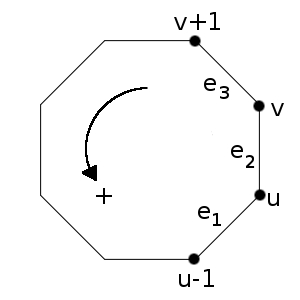
\includegraphics[scale=0.5]{GrapheCirculaire_PreuveSolutionEntiere.jpg}
  \caption{Notations pour la démonstration de la proposition \ref{Solution entière}}
  \label{Numerotation aretes parite}
\end{figure}

On résoud le programme mathématique \eqref{PLNE borne inf} relâché et on note $\bs{z} = (z_e)_{e \in E}$ la solution trouvée. On choisit deux sommets consécutifs $u,v \in U$ tels que $u$ et $v$ soient tout deux différents de $p$ et $q$. Quitte à renuméroter les arêtes, on peut supposer que $e_1 = (u-1,u)$, $e_2 = (u,v)$ et $e_3 = (v,v+1)$. (cf figure \ref{Numerotation aretes parite}.)

Avec les notations introduites dans la section \ref{Changement variables}, on a $\zeta_2~=~z(\delta(u))$ et $\zeta_3~=~z(\delta(v))$ qui sont paires selon la condition d'Euler et $\zeta_1~=~z(\delta({u,v}))$ qui est paire selon la relation de la proposition \ref{cout union}.

\`A l'aide de la forme explicite de la solution du système \eqref{Système linéaire extrait}, on en déduit que $z_1$ est entier, puis par une récurrence immédiate que $z_e$ est entier pour tout $e \in E$.
\end{proof}

